
\section{Unanswered questions and new physics quests}\label{sec:THquest}

The principal objection to the idea that the SM could be a final theory is the high number of parameters of the theory. In fact, 19 parameters are needed to fit data from experimental observations. 
Three of them  are the couplings of the gauge groups $g_3, g, g'$ also written as: \begin{equation}\label{eq:couplings}
\alpha_{s}=\dfrac{g_{3}^{2}}{4\pi} ,\quad \alpha_{elm} = \dfrac{e^{2}}{4\pi} =  \dfrac{g^{2}\sin^{2}\theta_{W}}{4\pi}, \quad \sin^{2}\theta_{W} = \dfrac{(g')^{2}}{g^{2}+(g')^{2}},
\end{equation}
13 parameters are associated with the nine charged fermion masses and the four parameters of the CKM matrix (three quark-mixing angles and one phase), two are needed to describe the SSB mechanism, i.e. the Higgs vacuum expectation value $v$ and the quartic coupling constant $\lambda$, and  finally one is the QCD $\theta$ parameter. Moreover, if neutrinos are massive (as it is almost certain from neutrino oscillation observations, see e.g. \cite{Langacker:817840}) there will be even more arbitrary parameters describing their masses and their mixing. Another disturbing feature of the model is the lack of theoretical explanation for the generations of quarks and leptons to be exactly three, and also the reason why particle masses are so different in order of magnitude is unknown.

Cosmology and cosmological observations also challenge the Standard Model. The reason for baryon-antibaryon asymmetry is still not understood although we know that it is connected to  CP violation. Besides, astronomical observations tell us that the energy density of the Universe is made only for a 4-5\% of ordinary baryonic matter, the other components being dark matter (20-25\%) and dark energy (70-76\%). Dark matter is non-baryonic matter that interacts only weakly and gravitationally. It is now believed that dark matter is composed  of Weakly Interacting Massive Particles (WIMPs) whose masses range from a few GeV to a few TeV and  are not predicted within SM. Dark energy instead is still more mysterious and maybe new physics will give some hints for its interpretation.

Another topic making the SM likely to need improvements is the desire to go further in the unification of theories. Gravity is not implemented in the SM being negligible at the electroweak scale of few hundreds of GeV, but it should become relevant going up to the Planck scale $\Lambda \sim 10^{19}$ GeV. Also, electroweak and strong forces forming the SM gauge group $SU(2)_{L}\otimes U(1)_{Y}\otimes SU(3)_{C}$ are expected to unify at high energy since their coupling constants are running constants dependent on the energy scale (Figure \ref{running}, $\alpha^{-1}_{i} = g^{2}_{i}/(4\pi)$). 
\begin{figure}[htb]\begin{center}
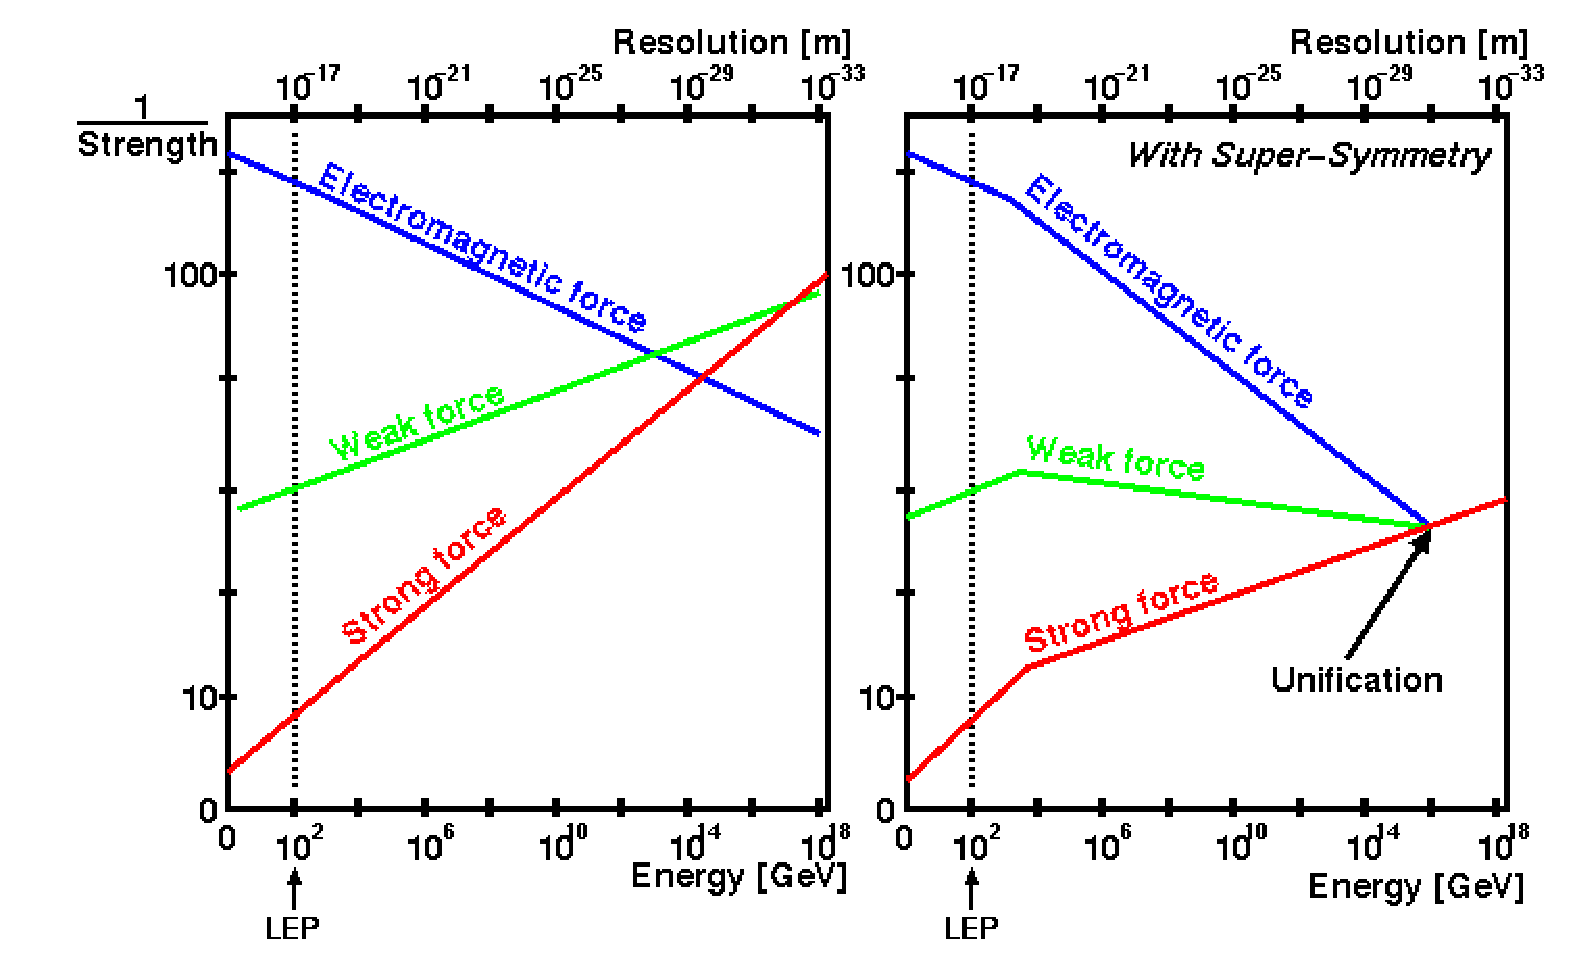
\includegraphics[width=.8\textwidth]{theory/figures/running_coupling}
\caption{Running coupling constants in the SM and in the MSSM (see Section \ref{sect:susy}) as functions of the renormalization scale (from \cite{pdg2008}).}
\label{running}\end{center}\end{figure}
If, based on these considerations,  one assumes that the Standard Model is valid only up to  an energy scale $\Lambda$, the scalar Higgs boson mass\footnote{This argument does not apply to fermion masses which are protected by chiral symmetry, and that's the reason why fermion masses are said to be ``natural''.} should encounter radiative corrections from vacuum polarization diagrams (Figure \ref{topLoop}) of the order of $\Lambda$ giving to the mass the value \cite{dawson-1997} \begin{equation}\label{eq:higgsMass}
M_{H}^{2} \sim M_{H_{0}}^{2} + \dfrac{\lambda}{4\pi^{2}} \Lambda^{2} + \delta M_{H}^{2}. \end{equation}
If the mass counterterm $\delta M_{H}^{2}$ does not cancel the quadratically divergent contribution and if the cutoff scale is chosen as the Planck scale, then
\begin{equation}
M_{H}^{2} \sim 10^{32},\end{equation} i.e. $10^{28}$ times bigger than the experimentally expected value coherent with the SM and with the unitarity constraint. This argument is called the \textit{hierarchy problem}, and could be fixed within the SM by choosing a fine-tuned mass counterterm, a solution considered not really elegant also because fine tuning will be required for every order in the perturbative expansion.
\begin{figure}[htb]\begin{center}
\includegraphics[width=.2\textwidth]{theory/figures/toploop}
\caption{The typical vacuum polarization diagram for the Higgs is a top quark loop.}
\label{topLoop}\end{center}\end{figure}
%This argument looks the same of what made physicists pass from Fermi theory to SM. In fact at that time the Fermi point like interactions were a good description of weak scattering processes of fermions $f+f\rightarrow f+f$, but the unitarity  predicted that at an energy $E_{crit} \sim 600$ GeV the theory would become inconsistent. Then it was found that new physics (the vector bosons of the SM) was needed already from an energy scale about 100 GeV, maybe due to the small coupling constant of weak interaction. Now, the scattering process $W+W\rightarrow W+W$ has a scattering amplitude growing linearly to the self-coupling constant of the Higgs field $\lambda$. The formula for the critical energy is now related to the Higgs mass as \cite{Ho-Kim} $$\dfrac{E_{crit}}{v} = \exp\bigg(\dfrac{4\pi^{2}v^{2}}{3M_{H}^{2}}\bigg),$$ which for an higgs Higgs mass less than 150 GeV gives $E_{crit} \sim 10^{18}$, thus making the Higgs model valid up to that scale. However for an heavier Higgs with a mass about 700 GeV, such critical energy goes down to $10^{3}$ GeV.  It is to remark that in the electroweak interactions the Higgs contribution to radiative corrections is very low since is denoted by a logarithm function, thus giving low variations and not affecting the precision electroweak data. The meaning of this is, whatever the critical energy value will be, the SM is an effective theory embedded in a more fundamental theory with $E_{crit}$ acting as a cutoff.



\subsection{Supersymmetry}

\subsection{Little Higgs}

\subsection{Extra-dimensions}

